\subsection{Web-Frontend}\label{Frontend}
\chapterauthor{Valentin Weiß}
Für das Projekt wurde ein Frontend geschaffen, in dem der Nutzer den ESP32 konfigurieren und Informationen auslesen kann.

\paragraph{Technologie}
\chapterauthor{Valentin Weiß}
Das Frontend wurde als Webseite mit Reactjs und Typescript implementiert.
Reactjs ist eines der bekanntesten und größten Javascript SPA (Single Page Application) Frontend Frameworks.
Typescript als Sprache bietet im Gegensatz zu Javascript Typsicherheit.
Dies verbessert die Codestabilität und die Lesbarkeit.
Weitere nennenswerte Pakete, welche für das Frontend benutzt werden, sind:
\begin{itemize}
    \item MUI: Eine bereits für React implementierte Version der Material Design Guidelines von Google. Für ein besseres \glqq look and feel\grqq.
    \item react-router-dom: Für das Routing zwischen den Unterseiten der Webseite.
    \item notistack: Für Benachrichtigungen in Form einer Snackbar.
    \item yup: Zur Validierung von Objekten
    \item react-hook-form: Zum Anzeigen von Fehlern und zur Verwaltung von Nutzereingaben.
    \item sass: Zur Einbindung von SCSS Dateien
\end{itemize}

\paragraph{Build Extension}
\chapterauthor{Valentin Weiß}
Durch das npm Paket \emph{react-app-rewired} ist es möglich, ohne den React Befehl \emph{eject} die Webpack Konfiguration von Reactjs in Teilen zu überschreiben.
Dadurch ist es möglich, in den Build Prozess zu einem gewissen Grad einzugreifen, und so die Komprimierung von Dateien per gzip zu aktivieren. Die Webseite hat ohne Komprimierung eine Größe von ca. 11 MB. Mit Komprimierung kann dies auf ca. 900 KB verringert werden. Dadurch ist es möglich die Webseite auf den doch sehr begrenzten Speicher des ESP zu laden.
Außerdem kann die Länge der Dateinamen beschränkt werden, da SPIFFS als verwendetes Dateisystem auf dem ESP nur eine Gesamtpfadlänge von 32 Bytes unterstützt.
Dies wird benötigt, da SPIFFS als Dateisystem nur eine Gesamtpfadlänge von 32 Bytes erlaubt und um den Speicherplatz des Webseitenkompilats auf weniger als 1 MB zu reduzieren.

\paragraph{Frontend Funktionsweise}
\chapterauthor{Valentin Weiß}
Das Web Frontend wird im Browser ausgeführt.
Das komprimierte Kompilat (bestehend aus mehreren Dateien) der React Anwendung muss daher vom ESP32 als statische Datei über eine Schnittstelle bereitgestellt werden.
Wir verwenden hierfür, und für die darauffolgende Datenabfrage eine REST Schnittstelle, welche über das HTTP Protokoll angesteuert wird.
Zunächst wird die index.html als Hauptdatei geladen.
In dieser sind Referenzen auf andere statische Dateien verlinkt, die somit nachgeladen werden können.
Am Ende wird der JavaScript-Code im Browser ausgeführt und über diesen benötigte Abhängigkeiten dynamisch nachgeladen.
React als ausführendes Framework erzeugt dann aus den berechneten, zu anzeigenden, JSX Komponenten eine internes virtuelles DOM als JSON.
Dieses zu HTML Code konvertiert und in das tatsächliche DOM eingefügt.
Im Fall einer Komponenten- oder Wertänderung kann so einfach das Unterelement der virtuellen DOM und dann das Element in der tatsächlichen DOM ausgetauscht werden.
Somit müssen nur minimale Teilelemente der WebUI neu geladen und gerendert werden und nicht die komplette Webseite.

\paragraph{Frontend Design}
\chapterauthor{Valentin Weiß}

\begin{figure}[htpb] % {H}
    \centering
    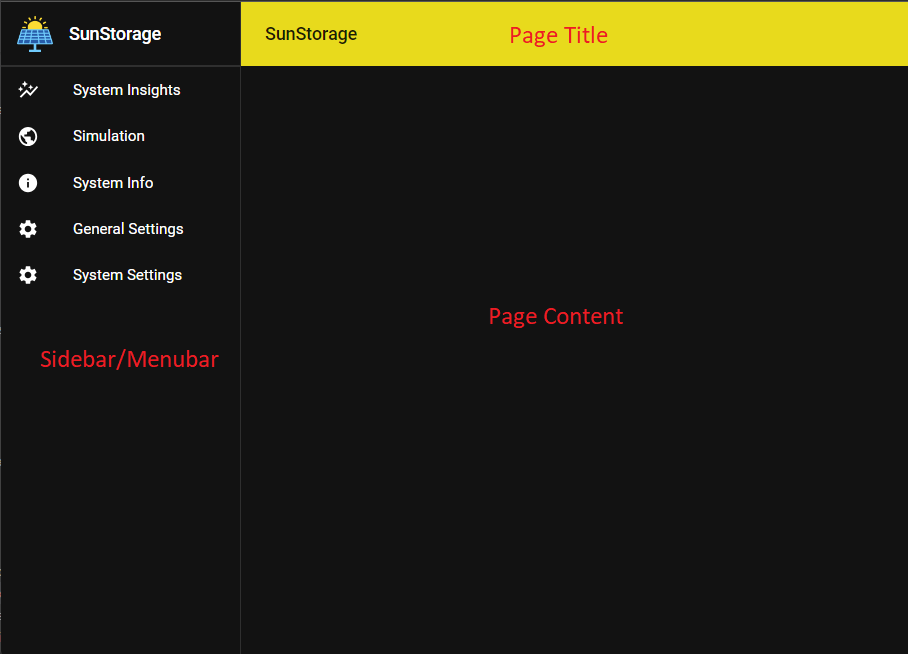
\includegraphics[width=\textwidth,keepaspectratio=true]{pics/Screenshot_Frontend_Design.png}
    \caption{Screenshot des Frontend Design}
    \label{fig:ScreenshotFrontendDesign}
\end{figure}

Wie in \autoref{fig:ScreenshotFrontendDesign} erkennbar, besteht das Frontend aus mehreren grundlegenden Komponenten. „Page Content“ ist die zentrale Komponente der Webseite  und zeigt die aktuell aufgerufene Seite an. „Page Title“ zeigt den Titel der Seite.
In „Sidebar/Menubar“ können die verschiedenen Seiten ausgewählt werden.
Dieses Menü verkleinert sich zu einem seitlich eingeschobenen Menü für kleine Displaybreiten und kann über einen Burger Button aufgerufen werden.
Das Menü bietet zudem die Funktion, je nach angezeigter Seite ein Untermenü einzubinden, um den „Page Content“ zu entlasten.
Dies ist vor allem für die in \autoref{websim} beschriebene Simulation wichtig.

\begin{figure}[htpb] % {H}
    \centering
    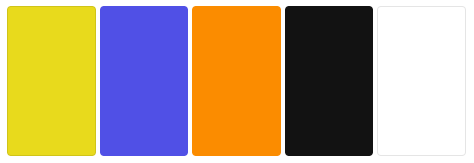
\includegraphics[width=\textwidth,keepaspectratio=true]{pics/Color_Palette_Frontend.png}
    \caption{Farbpalette}
    \label{fig:ScreenshotFrontendDesignColorPalette}
\end{figure}

Die Farbwahl (\autoref{fig:ScreenshotFrontendDesignColorPalette}) wurde passend zum Projektthema mit dem Spruch „Licht, das die Nacht erhellt“ als Kernthema entworfen. Ein mattes Gelb wurde somit als Primärfarbe gemeinsam mit einem dunklen Hintergrund definiert. Gelb als Farbe steht sowohl für die Sonne am Himmel, die auf das SolarPanel scheint als auch für den von unserem Gerät produzierten Strom. Eine nicht zu helle, matte Farbe zu wählen ist bei einem dunklen Hintergrund wichtig, damit kein stechender, greller Effekt für die Augen des Nutzers entsteht und komfortabel betrachtet werden kann.
Für die Schrift wurden Komplementärfarben zum aktuellen Hintergrund basierend auf der Farbpalette in \autoref{fig:ScreenshotFrontendDesignColorPalette} dargestellten verwendet. Ein mattes Lila als Sekundärfarbe zieht die Aufmerksamkeit des Nutzers nicht von den wichtigen Elementen der Seite weg und ist gut zu erkennen auf dem dunklen Hintergrund. Als abschließender Farbton wurde ein weiches Orange verwendet. Diese Farbe soll nur als weitere Option dienen, falls die Primär und Sekundäroptionen nicht ausreichen. Sie ist etwas intensiver als die Sekundärfarbe.

\subsubsection{Konfigurationsmöglichkeiten}
\chapterauthor{Valentin Weiß}

\begin{figure}[htpb] % {H}
    \centering
    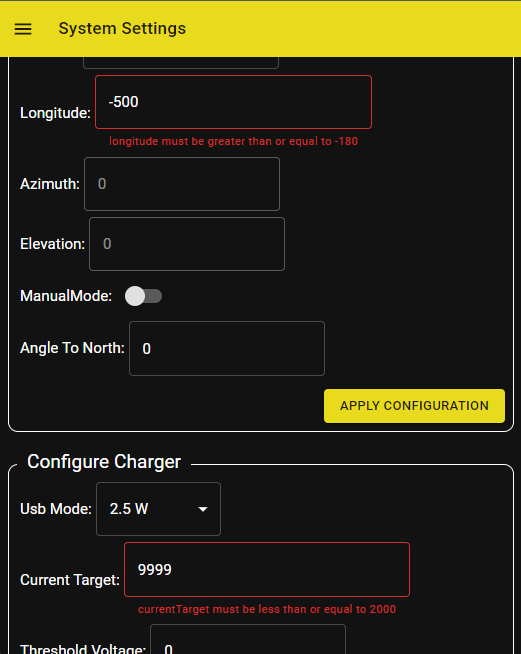
\includegraphics[height=12cm,width=\textwidth,keepaspectratio=true]{pics/Screenshot_SystemSettings.png}
    \caption{Screenshot der System Settings}
\end{figure}

Eine Kernfunktionalität ist die Konfiguration des SunStorage Systems. Hier bietet das Web-Frontend gruppenbasiert verschiedenste Konfigurationsmöglichkeiten zu folgenden Themen:
\begin{itemize}
    \item Positionierung und Panelausrichtung
    \item Ladegerät und Batterie
    \item Nachtabschaltung
    \item Display
    \item Stromsparen und zeitweise Abschaltung von Funktionen
    \item WiFi Konfiguration
\end{itemize}

Eingaben werden hier, wie auch auf allen anderen Seiten, auf Validität geprüft, um Datenintegrität zu gewährleisten und Missbrauch sowie potenziell gefährliche Konfigurationen zu vermeiden.
WiFi und Display werden nicht weiter aufgeführt.

\begin{table}[H]
    \begin{center}
      \begin{tabular}{|l|r|r|}
        \hline
        Wert          & Validierung & Beschreibung\\
        \Xhline{3\arrayrulewidth}
        Usb Mode & [0, 1, 2] & 0: 2.5 W; 1: 5 W; 2: 10 W \\
        \hline
        Current Target      & [0..2000]   & Wert in mA \\
        \hline
        Threshold Voltage   & [0..1000] & Wert in mV \\
        \hline
        Maximum Voltage   & [3800..4200] & Wert in mV \\
        \hline
        Trickle Threshold   & [3000..4200] & Wert in mV \\
        \hline
        Battery Size   & [0..10000] & Wert in mAh \\
        \hline
        Overheated Temperature   & [20..60] & Wert in Grad Celsius \\
        \hline
        High Power Enabled   & [true, false] &  \\
        \hline
        Overheated Hysteresis   & [1..10] & Wert in Kelvin \\
        \hline
      \end{tabular}
      \caption{Validierung Konfiguration Ladegerät}
    \end{center}
  \end{table}

  \begin{table}[H]
    \begin{center}
      \begin{tabular}{|l|r|r|}
        \hline
        Wert          & Validierung & Beschreibung\\
        \Xhline{3\arrayrulewidth}
        Enabled & [true, false] &  \\
        \hline
        Azimuth      & [0..360]   & Winkelgrad \\
        \hline
        Elevation   & [0..90] & Winkelgrad \\
        \hline
      \end{tabular}
      \caption{Validierung Konfiguration Nachtabschaltung}
    \end{center}
  \end{table}

  \begin{table}[H]
    \begin{center}
      \begin{tabular}{|l|r|r|}
        \hline
        Wert          & Validierung & Beschreibung\\
        \Xhline{3\arrayrulewidth}
        manualMode & [true, false] & Manuelle oder Automatische Panel Ausrichtung \\
        \hline
        Azimuth      & [0..360]   & Winkelgrad \\
        \hline
        Elevation   & [0..90] & Winkelgrad \\
        \hline
        Latitude   & [-90..90] & Breitengrad \\
        \hline
        Longitude   & [-180..180] & Längengrad \\
        \hline
        Angle To North   & [0..360] & Winkelgrad \\
        \hline
      \end{tabular}
      \caption{Validierung Konfiguration Positionierung}
    \end{center}
  \end{table}

  \begin{table}[H]
    \begin{center}
      \begin{tabular}{|l|r|r|}
        \hline
        Wert          & Validierung & Beschreibung\\
        \Xhline{3\arrayrulewidth}
        HTTP & [0..] & in Sekunden \\
        \hline
        GPS & [0..] & in Sekunden \\
        \hline
        WiFi & [0..] & in Sekunden \\
        \hline
        DCF-77 & [0..] & in Sekunden \\
        \hline
      \end{tabular}
      \caption{Validierung Konfiguration Funktionsabschaltung}
    \end{center}
  \end{table}

Eine Verbesserung der Displaykonfiguration wäre gewesen, wenn man nicht nur verschiedene Werte auf dem Display aktivieren und deaktivieren, sondern auch die Reihenfolge anpassen könnte. Dies wird jedoch von der API nicht unterstützt.

\subsubsection{System Insights}
\chapterauthor{Valentin Weiß}

\begin{figure}[htpb] % {H}
    \begin{center}
    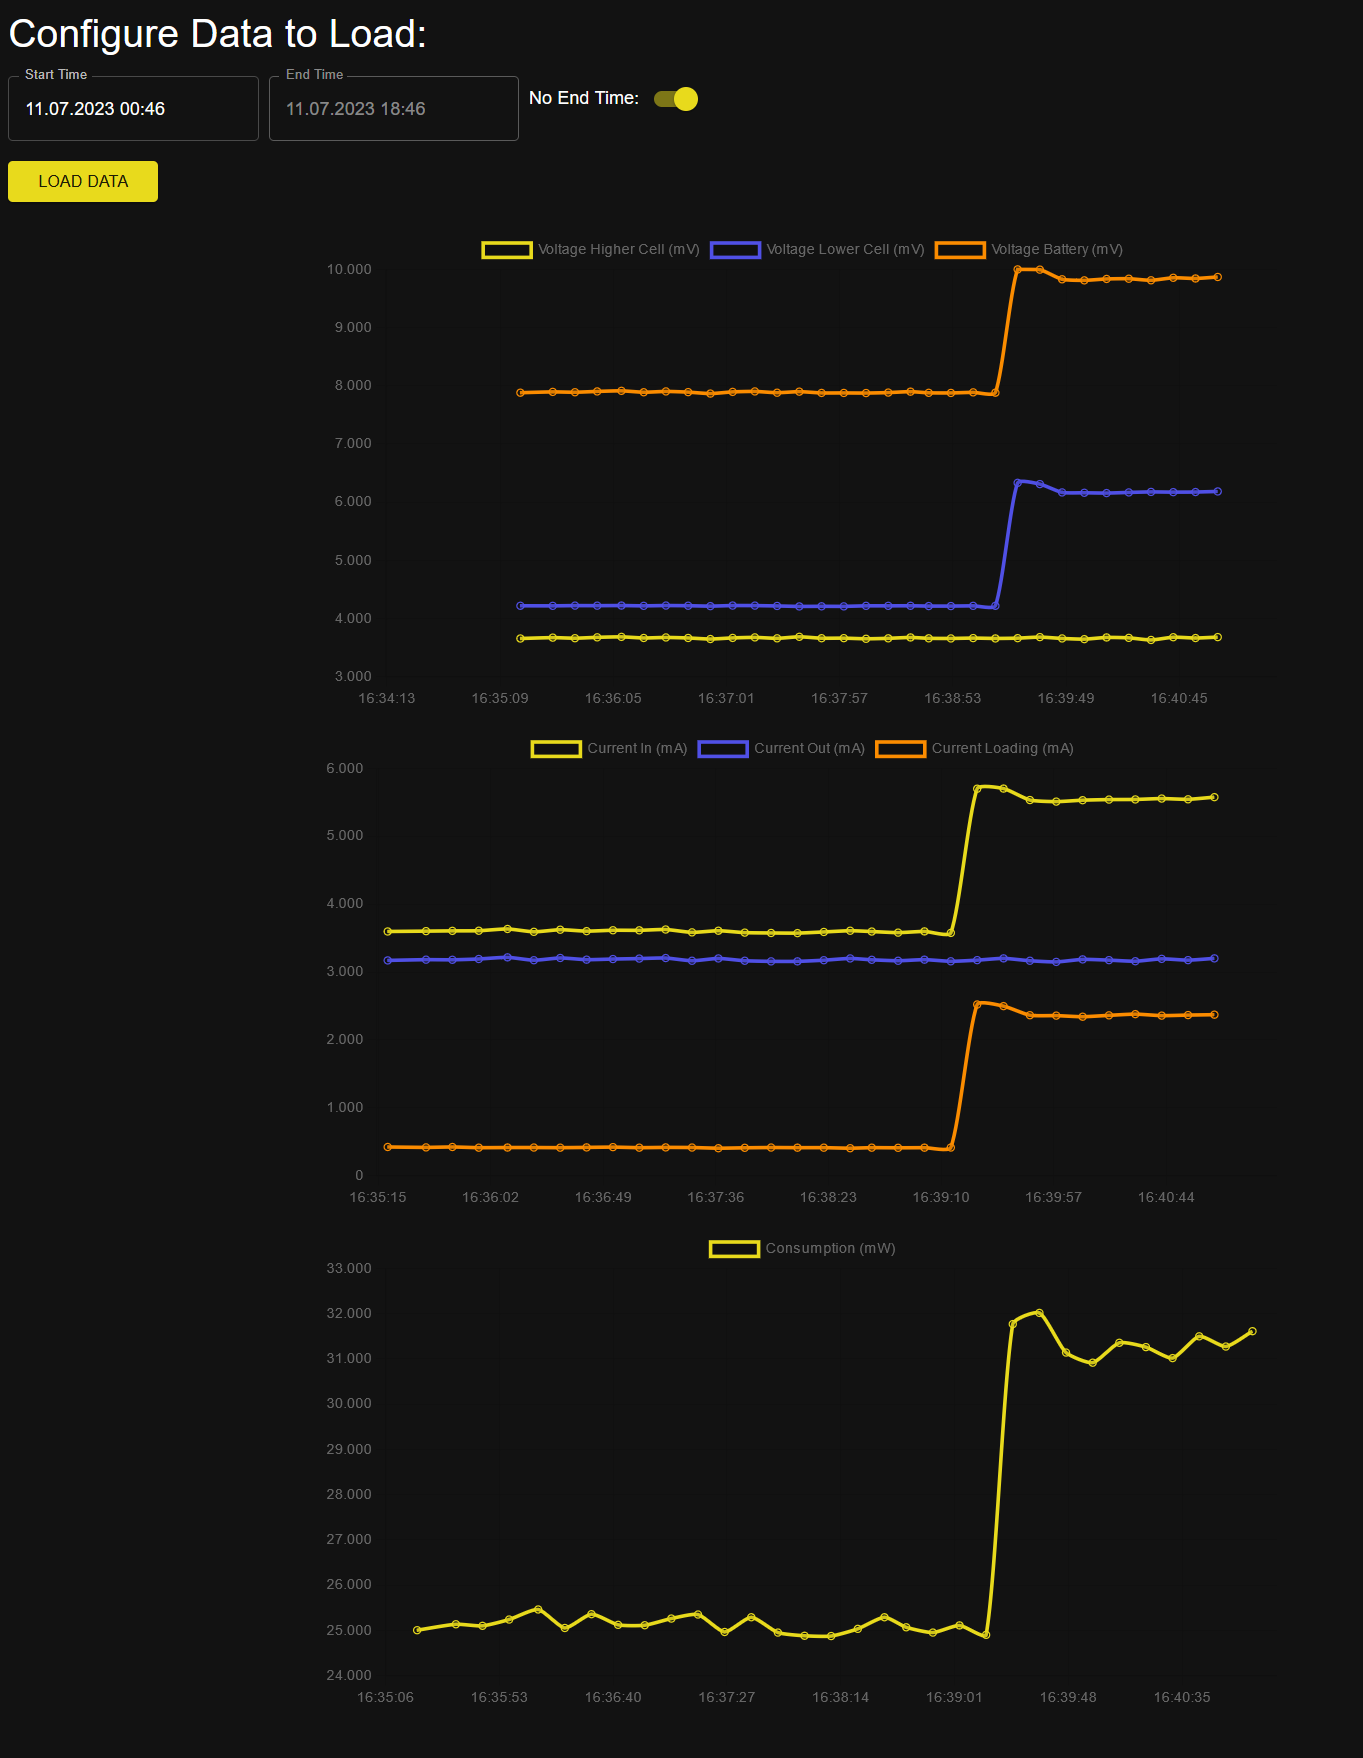
\includegraphics[width=10cm,keepaspectratio=true]{pics/Screenshot_ApplicationInsights.png}
    \caption{Screenshot der System Insights}
    \label{fig:systeminsights}
	\end{center}
    Der Sprung in den Werten entsteht durch das in die Sonne stellen.
   	In den finalen Einstellungen ist die Abtastrate wesentlich niedriger.
   	Auf die Richtigkeit der Werte wird in Kapitel \autoref{akkuCircuit} eingegangen.
   	Durch Messungen stellte sich heraus, dass der Bipolartransistor zur Steuerung des Ladestroms kaputt ist.
   	Daher wird der Ladestrom nicht gesteuert.
\end{figure}

Diese Seite bietet, wie in \autoref{fig:systeminsights} gezeigt, die Möglichkeit Systemdaten über einen Zeitbereich auszulesen und sie graphisch darzustellen.
Hier können entweder Datensätze über einen Zeitbereich zwischen einer Start- und Endzeit oder zwischen Startzeit und dem neusten verfügbaren Datensatz ausgelesen werden.
Es werden drei Graphen gebildet:
\begin{enumerate}
    \item Graph für Spannungsinformationen
    \item Graph für Strominformationen
    \item Graph für Leistungsinformationen
\end{enumerate}

Dies wurde mittels der react-chartjs-2 Bibliothek umgesetzt, die eine React Implementierung für das chart.js Framework bietet.

\subsubsection{Ungenutzte Erweiterungen}
\chapterauthor{Valentin Weiß}
Da das Frontend schon sehr früh im Projekt implementiert wurde, sind später Funktionalitäten hinzugefügt worden, welche die User-Experience weiter verbessern.
Aus zeitlichen Gründen konnten diese nicht im Backend umgesetzt werden.
Dies beinhalteten hauptsächlich das Streaming von Informationen.
Hierfür wurden zwei ungenutzte Technologien implementiert.

\paragraph{HTTP SSE (Server-Sent Events)}
\chapterauthor{Valentin Weiß}

SSE bietet die Möglichkeit über offene HTTP Verbindungen Daten vom Server zum Client zu senden.
Hier wäre es möglich gewesen, aktuelle Datenänderungen direkt an das Frontend zu streamen, ohne dass ein Client Änderungen anfragen muss.
Eine Entlastung des ESP kommt hier zustande, wenn mehrere Frontendinstanzen die gleichen Daten regelmäßig abfragen, um möglichst aktuell zu bleiben.
Hiermit könnte man beispielsweise in Application Insights Diagramme erstellen, die die neusten Werteveränderungen über die Zeit direkt anzeigen.

\paragraph{MQTT (Message Queuing Telemetry Transport)}
\chapterauthor{Valentin Weiß}
Die MQTT Implementierung hätte ähnlich wie SSE verwendet werden können, um im Frontend mit aktuellen Daten zu arbeiten, ohne den ESP weiter zu belasten.
Der ESP sendet die neuen Daten an einen Broker, welcher die Verteilung von Daten übernimmt.
Dadurch wäre der ESP von Anfragen entlastet, da diese der Broker als externes Gerät übernimmt.
Besonders dann, wenn mehrere Frontend-Clients gleichzeitig verwendet werden.
Diese Technologie gilt als Standard im IoT Bereich \autocite{front:mqtt}.

\paragraph{Web Logging}
\chapterauthor{Valentin Weiß}
Durch eine SSE oder MQTT Realisierung wäre es möglich das umgesetzte Web Logging zu verwenden.
Hier hätten Log Nachrichten des ESP live ausgelesen und angezeigt werden können, was beim Debugging hilfreich gewesen wäre.
Durch die Belegung eines UART Ports des ESP durch das GPS Modul muss nach dem Zusammenbau des Projekts muss das Logging über UART deaktiviert sein.
Besonders in dieser letzten Phase des Projekts wäre das Web Logging hilfreich gewesen.
Eine weitere Möglichkeit ist, ein Logfile auf der SD-Karte des ESP zu erzeugen, um die Daten per HTTP auszulesen.
Auch diese Funktion wird vom ESP aktuell nicht unterstützt.

\subsubsection{Fazit}
\chapterauthor{Valentin Weiß}
Insgesamt war es sehr interessant das Web-Frontend zu planen und zu Implementieren.
Ich habe nun ein guts Verständnis von React Anwendungen und habe mein bisheriges Wissen in den Webtechnologien weiter vertieft.
Da dieses Framework doch sehr anders funktioniert als bisher benutzte Technologien habe ich länger als geplant zur Einarbeitung und zum Lernen der Umgebung benötigt.
Neue Konzepte wie React Context, Hooks oder die komponentenbasierte Projektverwaltung sind sehr interessant.

Vergleichsweise häufige API Änderungen verursachten zusätzlichen Zeitaufwand, welcher durch mehr Kommunikation und Planung vermeidbar gewesen wäre.
Obwohl viel Code am Ende ungenutzt bleibt, hat mich die Einarbeitung in MQTT und SSE persönlich weitergebracht.

Insgesamt bin ich zufrieden mit dem Ergebnis des Web-Frontend.

\subsection{Simulation des Panels im Frontend}\label{websim}
\chapterauthor{Valentin Weiß}
Das Web-Frontend soll dem Nutzer die Möglichkeit bieten, über eine 3D Simulation die Sonnenposition und Panelausrichtung darzustellen, damit sich der Nutzer die Ausrichtung und Zusammenhänge besser vorstellen kann.

\subsubsection{Sky Dome Model}
\chapterauthor{Valentin Weiß}
Wegen der großen Entfernung der Sonne zur Erde von knapp 150 Millionen Kilometern wird die Sonne nur als helle, kleine Kreisfläche wahrgenommen.
In einem Kuppelmodell (Sky Dome Model) machen wir uns das zu nutze (\autoref{fig:DomeModel}).
In diesem Modell wird eine Position auf der Erde annähernd als Kreisfläche dargestellt. Die Sonne (oder auch andere Objekte im Weltall) wird hier in konstanter Distanz auf der Kuppel in der echten Richtung dargestellt. Dies ist natürlich von verschiedenen Faktoren wie Ort und Zeit abhängig.

\begin{figure}[htpb] % {H}
    \centering
    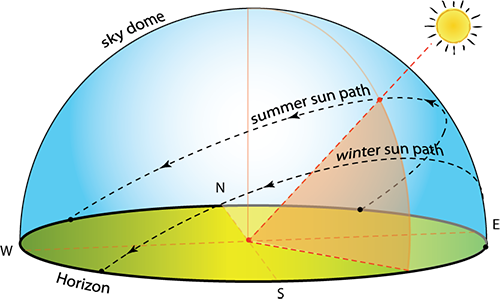
\includegraphics[width=\textwidth,keepaspectratio=true]{pics/SkyDomeModel.png}
    \caption{Simulation Model: SkyDome \autocite{front:SkyDome:img}}
    \label{fig:DomeModel}
\end{figure}

\subsubsection{Algorithmus Sonnenposition}

\paragraph{Grundlegender Algorithmus}
\chapterauthor{Valentin Weiß}

Für die Simulation, aber auch für die automatische, optimale Panelausrichtung auf dem ESP muss die Position der Sonne berechnet werden.
Wie im Simulationsmodell (\autoref{fig:DomeModel}) gezeigt, muss der Drehwinkel (Azimut) sowie der Steigungswinkel (Elevation) zur Sonne über einen Algorithmus berechnet werden.

Azimut ist hierbei der Drehwinkel auf durch die Erdoberfläche dargestellten Ebene.
Dieser zeigt mit $0\degree$ Richtung Norden und dreht sich bei steigenden Werten gegen den Uhrzeigersinn. Beispielsweise zeigt ein Azimut von $90\degree$ Richtung Westen. Der Wertebereich des Azimut liegt somit bei $[0\degree; 360\degree]$ \autocite{front:AzimuthAngle}.

Elevation ist der Winkel, der aussagt, wie weit die Sonne über oder unter dem Horizont steht. In Abbildung \ref{fig:DomeModel} ist dieser Winkel in der Farbe orange eingetragen.
Ein Winkel größer als $0\degree$ sagt aus, dass die aktuelle Position beleuchtet ist (Tag). Ein Winkel kleiner als $0\degree$ bedeutet, dass die Sonne die aktuelle Position nicht beleuchtet (Nacht).
Beispielsweise repräsentiert $0\degree$ den Sonnenaufgang oder Sonnenuntergang.
$90\degree$ beschreibt, dass die Sonne direkt über der aktuellen Position ist.
Der Wertebereich der Elevation liegt somit bei $[-90\degree; 90\degree]$ \autocite{front:ElevationAngle}.

Die Sonnenposition an gewissen Koordinaten ist abhängig von der Erdrotation zur Sonne.
Diese kann durch den Stundenwinkel $HRA$ (Hour Angle) an einer Position bzw. gewissen Koordinaten dargestellt werden.
Der Stundenwinkel $HRA$ ist der Verlauf der Sonne, den man an einem gewissen Tag an einer gewissen Position wahrnimmt.
Dabei wird der höchste Stand der Sonne (Solar Noon) mit $0\degree$ definiert. Durch die Drehung der Erde von $15\degree$ pro Stunde ($\frac{360\degree}{24h} = \frac{15\degree}{1h}$), ändert sich auch der Stundenwinkel pro Stunde um diesen Wert. Ein negativer Winkel repräsentiert einen Winkel vor dem Höchststand der Sonne, ein positiver einen Winkel nach dem Höchststand der Sonne. Beispielsweise ist ein $HRA$ Winkel von $-45\degree$ einer Zeit 3 Stunden vor dem Sonnenhöchststand zugeschrieben \autocite{front:SolarTime}.

Die lokale Sonnenzeit $LST$ (Local Solar Time) bestimmt mit der Uhrzeit 12:00 Uhr genau diesen Winkel ($HRA = 0\degree$) und somit eine einfache Berechnung des Winkels:

\[ HRA = 15\degree*(LST - 12) \]

Der Sonnenhöchststand ist etwa Mittags $LT$ (lokale Zeit/Local Time), jedoch muss es aufgrund der Ungenauigkeit der Zeitzonen gegenüber der Position im Längengrad ($TCLongitude$) und der Ungenauigkeit der Erdumlaufbahn zur Sonne inklusive Achsenwinkel ($TCEoT$) ein zeitlicher Korrekturfaktor in Minuten $TC$ (Time Correction Factor) zur $LT$ addiert werden, um die $LST$ zu berechnen.

\[ LST = LT + \frac{TCLongitude + TCEoT}{60} \]

\[ TCLongitude = \frac{4min}{1\degree}*(Longitude - (\frac{15\degree}{1h} * T_{UTC})) \]

Wobei sich die Erde um 15 Grad pro Stunde und folgend um 1 Grad alle 4 Minuten dreht. $T_{UTC}$ ist die Zeitzone, in der man sich befindet in Stunden abhängig von der koordinierten Weltzeit $UTC$ (Coordinated Universal Time). Für Deutschland ist diese Zeitzone im Winter MEZ ($UTC+1$) und im Sommer MESZ ($UTC+2$).

\[ TCEoT = 9.87sin(2B) - 7.53cos(B) - 1.5sin(B) \]

Wobei

\[ B = \frac{360\degree}{365\,days\,per\,Year}*(d - 81) \]

$d$ ist hierbei der Tag im aktuellen Jahr ab dem ersten Januar. $81$ ist der 81te Tag im Jahr, also der 22. März. An diesem Tag steht die Erde zur Sonne im Neigungswinkel $0\degree$ (\autoref{fig:DeclinationAngleFigure}). Je nach Schaltjahr könnte hier ein genauerer Wert verwendet werden, jedoch ist die $TCEoT$ (Equasion of Time) Abweichung so gering, dass das dies nur einen geringen Einfluss auf mehrere Nachkommastellen hätte, wordurch dies zu vernachlässigen ist. Der durch diese empirische Gleichung berechnete Wert ($TCEoT$) auch nur eine Annäherung die auf etwa eine halbe Minute genau ist.

\begin{figure}[htpb] % {H}
    \centering
    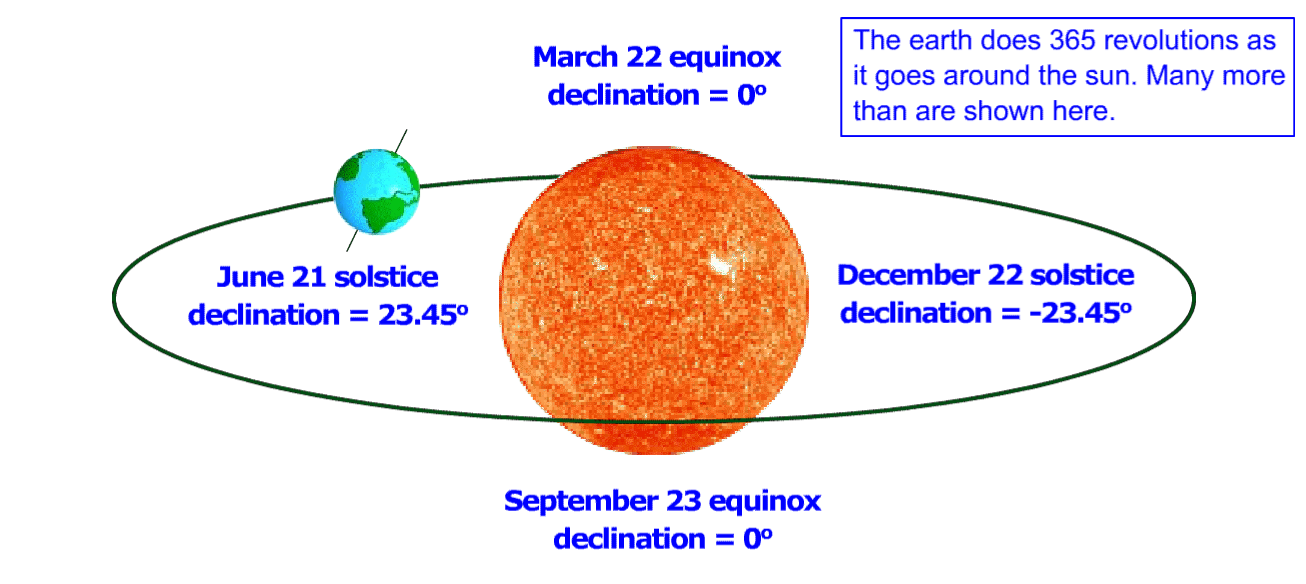
\includegraphics[width=\textwidth,keepaspectratio=true]{pics/DeclinationAngleEarthSun.png}
    \caption{Darstellung des Erdwinkel zur Sonne \autocite{front:DeclinationAngle}}
    \label{fig:DeclinationAngleFigure}
\end{figure}

\begin{figure}[htpb] % {H}
    \centering
    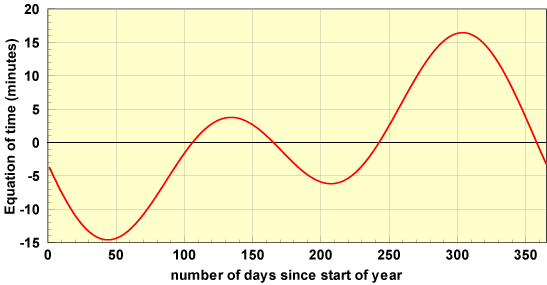
\includegraphics[width=\textwidth,keepaspectratio=true]{pics/TCEoT.png}
    \caption{Darstellung der Werte von $TCEoT$ über das Jahr \autocite{front:SolarTime}}
    \label{fig:TCEoT}
\end{figure}

Nachdem nun der $HRA$ Wert berechnet werden kann, muss die Neigung der Erdkugel zur Sonne noch berücksichtigt werden. Diese Neigung $\delta$ berechnet sich aus der maximalen Erdneigung von $23.45\degree$ in Kombination mit einer Sinusfunktion der bereits zuvor erklärten $0\degree$ Neigung am 22. März \autocite{front:DeclinationAngle}.

\[ \delta = 23.45\degree * sin(B) \]

$\delta$ kann als eine nördliche/südliche Äquator-Verschiebung gesehen werden, an der die Sonne im Elevationswinkel von $90\degree$ zur $LST$ 12:00 Uhr scheint.

$Azimut$ und $Elevation$ berechnen sich durch die kombination der zuvor berrechneten Werte:

\[ Elevation = sin^{-1} \left[sin(\delta)*sin(Latitude) + cos(\delta)*cos(Latitude)*cos(HRA)\right] \]

\[ Azimut = cos^{-1} \left[\frac{sin(\delta)*cos(Latitude) - cos(\delta)*sin(Latitude)*cos(HRA)}{cos(Elevation)}\right] \]

Die obere Berechnung gibt den korrekten Wert nur für Zeiten vor dem Höchststand der Sonne. Für den fall, dass $HRA > 0$ oder $LST > 12$ muss der $Azimut$ von $360\degree$ abgezogen werden.

\[ Azimut = 360\degree - Azimut \]

\paragraph{Verbesserungen den Algorithmus für die Simulation}
\chapterauthor{Valentin Weiß}

Der Algorithmus funktioniert gut, um eine statische Sonnenposition zu berechnen, jedoch hat dieser Probleme, wenn es darum geht die Sonne zu simulieren, da vor allem beim Übergang der Animation von einem Tag zum darauffolgenden unschöne Sprünge der Sonne auftreten können.

\begin{enumerate}
    \item Bei der Berechnung des Tags im aktuellen Jahr wurden statt Ganzzahlen nun Fließkommazahlen verwendet. Die verringert Sprünge in der Position beim Anbruch eines neuen Tages.
    \item Es kann vorkommen, dass die $LST$ negativ ist, in der Nähe der Mitternachtszeit. Dies tritt beispielsweise auf, wenn der berechnete zeitliche Korrekturfaktor $TC$ negativ ist und $LT$ klein ist (neuer Tag). Deshalb wird der Wert $LST$ auf das Intervall $[0h; 24h]$ normalisiert nach der Berechnung.
    \item Der Winkel $HRA$ verursacht auch Probleme der gleichen Art. Auch dieser musste auf ein festes Intervall von $[-180\degree; 180\degree]$ normalisiert werden.
\end{enumerate}

Durch diese Verbesserungen ist es möglich, die Sonne in der Simulation durchwegs flüssig und ohne Sprünge zu animieren.

\subsubsection{Positionierung im 3D-Raum}
\chapterauthor{Valentin Weiß}

Um das Simulationsmodell Sky Dome zu realisieren, muss zunächst ein 3D-Raum definiert werden. Da der Beobachter der Simulation bzw. das SolarPanel immer ein Eckpunkt der folgenden Berechnungen sein wird, ist es sinnvoll diesen an den Ursprung der Simulation zu positionieren. So sind die Koordinaten eines Punktes auch immer der Vektor vom Ursprung zum Punkt. Ein Punkt in diesem 3D-Raum $P(x,y,z)$ soll folgendermaßen definiert sein:
\begin{itemize}
    \item $x$ Achse: West-Ost Achse im Sky Dome Model. Mit $x < 0$ Westrichtung und $x > 0$ Ostrichtung.
    \item $y$ Achse: Oben-Unten Achse im Sky Dome Model. Mit $y < 0$ als „Unten“ und $y > 0$ als „Oben/Himmel“.
    \item $z$ Achse: Nord-Süd Achse im Sky Dome Model. Mit $z < 0$ Nordrichtung und $z > 0$ Südrichtung.
\end{itemize}

\paragraph{Sonnenposition im 3D-Raum}
\chapterauthor{Valentin Weiß}

Eine der wichtigsten Funktionen der Simulation ist, die Sonne anhand den berechneten Winkeln Azimut und Elevation richtig zu positionieren. Ein Vektor der Länge 1 würde mit den Winkeln $Azimut = 0\degree$ und $Elevation = 0\degree$ nach obriger Definition folgendermaßen aussehen:

\[
\mathbf{v} = \begin{bmatrix}
x \\
y \\
z \\
\end{bmatrix}
=
\begin{bmatrix}
0 \\
0 \\
-1 \\
\end{bmatrix}
\]

Dieser Vektor zeigt also eine Einheit Richtung Norden. Um die Richtung dieses Vektors anhand beliebiger Winkel für $Azimut$ und $Elevation$ anzupassen, muss der Vektor anhand der für den $Azimut$ Winkel an der y-Achse gegen den Uhrzeigersinn gedreht werden. Anschließend für den $Elevation$ Winkel an der daraus resultierenden Senkrechten durch den Ursprung. Um dies Programmtechnisch einfacher und ohne mehrmalige Rotationsmatrizen umzusetzen wurde der Fakt genommen, der oben genannte Eingangsvektor bekannt ist und am Ursprung anliegt, um dies mit einfachen Trigonometrischen Funktionen zu lösen.

\[
\mathbf{v} = \begin{bmatrix}
x \\
y \\
z \\
\end{bmatrix}
=
\begin{bmatrix}
cos(elevation) * sin(azimut) * -1 \\
sin(elevation) \\
cos(elevation) * cos(azimut) * -1 \\
\end{bmatrix}
\]

Dieser repräsentiert nun einen Vektor der Länge 1, der in Richtung der Sonne zeigt. Dieser kann jetzt einfach mit einer Konstante multipliziert werden, um als Punkt gesehen die Koordinaten der Sonne in Entfernung der Konstanten zu bestimmen.

\paragraph{SolarPanel Ausrichtung und Effizienzberechnung}
\chapterauthor{Valentin Weiß}

Die SolarPanel Ausrichtung erfolgt wie bei der Sonne über die Winkel $Azimut$ und $Elevation$. Hier muss nur anschließend die Höhe der Panel-Halterung auf den y-Wert addiert werden, damit das Panel durch die Höhe der Halterung keine Ungenauigkeit bekommt. Um die Form in Richtung Sonne zeigen zu lassen sind keine weiteren Berechnungen nötig, da diese Funktion bereits in der Three.js Bibliothek existiert.

Die Effizienzberechnung in der Simulation ist eine rein ausgedachte Methode, kann aber annähernd als guter Referenzwert angenommen werden.
Sei $\mathbf{v}_{\mathrm{1}}$ der Vektor zur Sonnenposition und $\mathbf{v}_{\mathrm{2}}$ die Blickrichtung des SolarPanels, dann ist der Winkel $\alpha$ zwischen den beiden Vektoren:

\[
\alpha = \cos^{-1} \left[\frac{\mathbf{v}_{1} \cdot \mathbf{v}_{2}}{|\mathbf{v}_{1}| \cdot |\mathbf{v}_{2}|}\right]
\]

Dann ist die Effizienz des SolarPanels wenn $\alpha < 90\degree$ und $Elevation > 0$

\[
Effizienz = cos(\alpha) * 100\%
\]

an sonsten $0\%$. Somit bringt das SolarPanel bei kleinen Winkelverschiebungen immer noch hohe Effizienzwerte, ist jedoch nach Sonnenuntergang bzw. ab einem abweichenden Winkel von über $90\degree$ $0\%$, da keine aktive Beleuchtung nicht mehr stattfindet.

\subsubsection{Umsetzung der Simulation}

\paragraph{Simulationsmenü}
\chapterauthor{Valentin Weiß}

Wie aus dem Algorithmus hervorgeht, werden verschiedene Parameter für die Simulation benötigt, um mit dem Algorithmus die Sonnenposition berechnen zu können.
Um diese Anforderungen visuell umzusetzen, ohne viel Platz für die Simulation zu verbrauchen, wurde ein Untermenü geschaffen, welches das eigentliche Menü mit Funktionen erweitert. Der Datenaustausch zwischen Simulation und Menü erfolgt über einen React Context.

Einstellungen Zur Berechnung der Sonnenposition in diesem Modell sind:
\begin{itemize}
    \item Längengrad und Breitengrad: Die Sonnenposition ist abhängig davon wo man sich auf der Erdkugel befindet. Je nach Position kann es verschiedene Sonnenstände zur gleichen Uhrzeit geben.
    \item Datum: Über das Jahr gesehen (abhängig von der Erdwinkel zur Sonne) verändert sich die Sonnenposition.
    \item Uhrzeit + Zeitzone: Die Erdrotation zur Sonne ist abhängig von Uhrzeit und Zeitzone.
\end{itemize}

Einstellungen zur Position des SolarPanels in der Simulation:
\begin{itemize}
    \item Azimut Winkel: Winkel zur Rotation des SolarPanels am Boden.
    \item Elevation Winkel: Winkel zur Neigung des SolarPanels.
    \item "Best Panel Angle": Diese Option deaktiviert die Bearbeitung von Azimut und Elevation. Diese Felder werden automatisch mit den optimalen Stand zur Sonne gefüllt.
\end{itemize}

Simulationsanimation:
\begin{itemize}
    \item „Animation Speed“: Wenn in diesem Feld eine Zahl steht, wird pro Sekunde in Simulationszeit die Sonne um X Minuten simuliert. Beispielwert 60: Pro Sekunde Simulation = 1 Stunde Sonnenverschiebung. Auch negative Werte sind möglich.
\end{itemize}

 Über die „Show Simulation Info“ Option werden live Werte der Sonnenberechung sowie die berechnete Effizienz des SolarPanel ausgegeben.

 \begin{figure}[htpb] % {H}
    \centering
    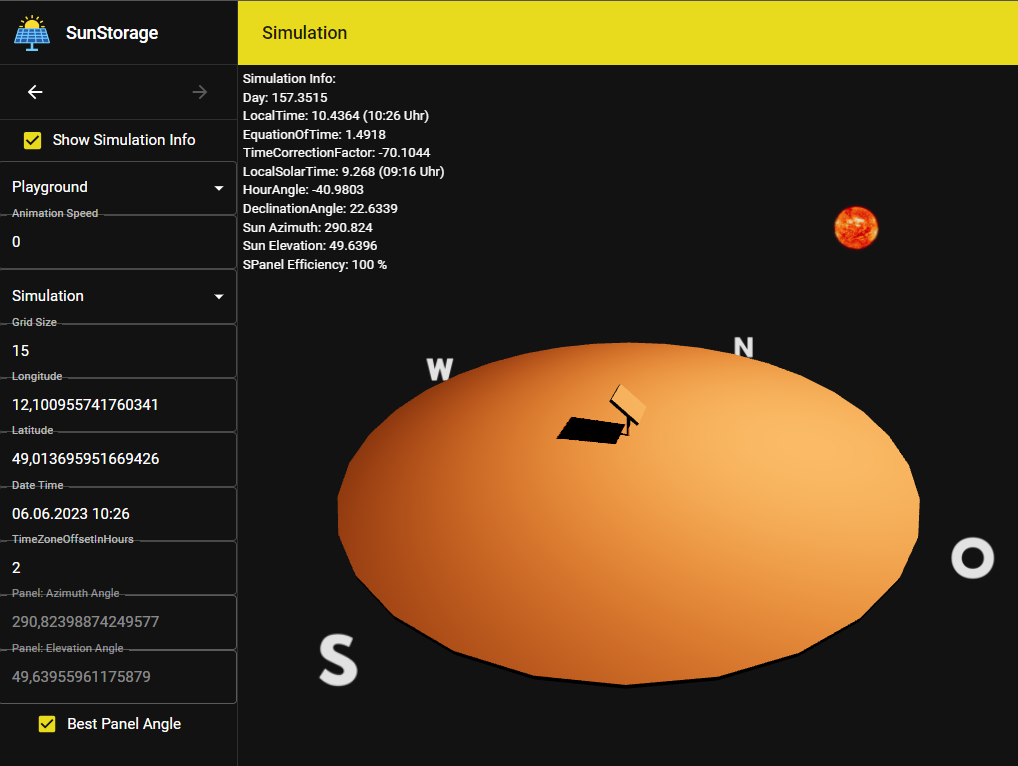
\includegraphics[width=\textwidth,keepaspectratio=true]{pics/Screenshot_WebUI_Simulation.png}
    \caption{Screenshot des Simulation Playground}
    \label{fig:SimulationScreenshotPlayground}
\end{figure}

\begin{figure}[htpb] % {H}
    \centering
    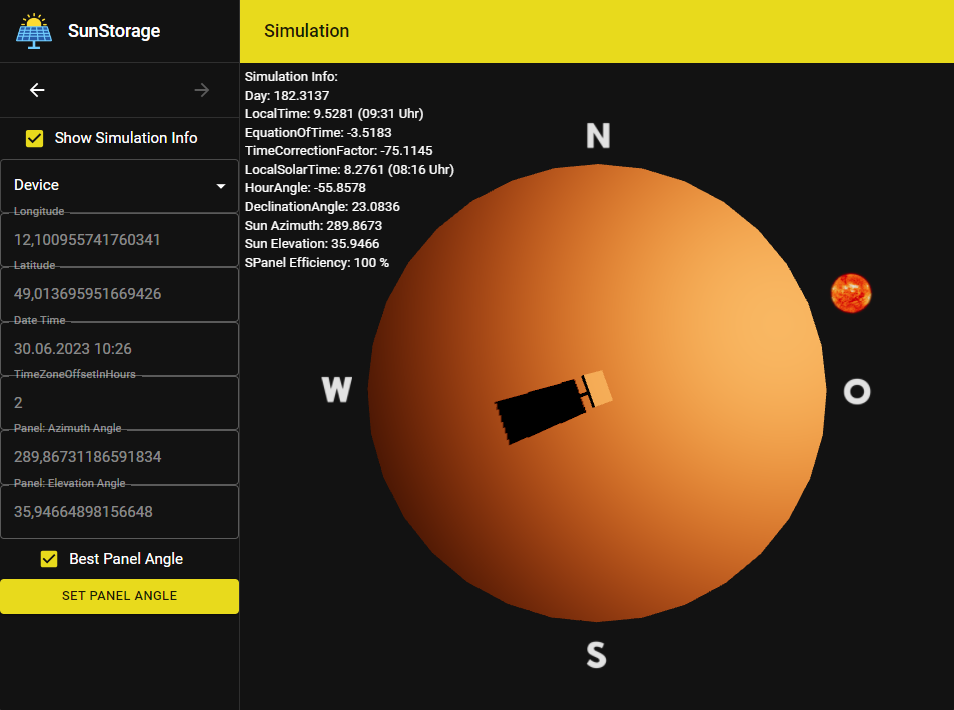
\includegraphics[width=\textwidth,keepaspectratio=true]{pics/Screenshot_WebUI_Simulation_Device.png}
    \caption{Screenshot des Simulation Device}
    \label{fig:SimulationScreenshotDevice}
\end{figure}

 Es wurden 2 Modi für die Konfiguration geschaffen.
 Im Modus Playground (Abbildung \ref{fig:SimulationScreenshotPlayground}) sind erweiterte Einstellungen für die Simulation möglich, wie beispielsweise die manuelle Eingabe der Koordinaten, der Zeit und Zeitzone sowie eine Option, die Zeit in beliebiger Geschwindigkeit zu animieren, um den Sonnenverlauf besser zu betrachten.
 Im Modus Device (Abbildung \ref{fig:SimulationScreenshotDevice}) ist nur die Einstellung des SolarPanel möglich, kombiniert mit einem zusätzlichen Button diese Konfiguration an das Gerät zu senden.

Eine weitere Verbesserung, die aufgrund von Zeitgründen nicht mehr implementiert wurde, ist das mit Einbeziehen des Standwinkels vom SunStorage Gerät, um eine Winkelkorrektur des SolarPanels zur Sonne an unebenen Flächen zu gewährleisten. Dies wurde nun nur auf dem ESP implementiert.

\paragraph{Simulationsanimation}
\chapterauthor{Valentin Weiß}

Die Simulation wurde mithilfe von Three.js implementiert. Three.js ist eine JavaScript-Bibliothek, die zum Erstellen und Anzeigen animierter 3D-Grafiken benutzt wird. Durch das Verwenden von WebGL wird die Grafikkarte angesteuert, um hohe Aktualisierungsraten und somit flüssige Animationen zu erstellen.
Um die Integration von Three.js in React zu erleichtern und zu erweitern, wurden folgende Bibliotheken verwendet:
\begin{itemize}
    \item @react-three/fiber: Ein React Renderer für Three.js
    \item @react-three/drei: Funktionserweiterungen und Abstraktionen von @react-three/fiber
\end{itemize}

\subsubsection{Fazit Simulation}
\chapterauthor{Valentin Weiß}

Insgesamt war die Simulation mein persönliches Highlight des ganzen Projekts. Eine interessante Kombination aus Mathematik und dem Arbeiten im 3D Raum. Obwohl ich viele Stunden in die Simulation gesteckt habe, war die Umsetzung doch einfacher als erwartet durch ein exzellentes Framework (Three.js) und hierfür bereits existierende Implementierungen und Erweiterungen für React Projekte.

Der Algorithmus zur Berechnung der Sonnenposition hat dafür länger als erwartet gedauert. Hierfür musste ich verschiedene Algorithmen, Quellen und Pakete untersuchen, welche oft nicht zum erwarteten Ergebnis geführt haben.
